\section{}
% onsider a modified form of Couette flow in which there are two immiscible 
% fluids sandwiched between two infinitely long and wide, parallel flat plates. The 
% flow is steady, incompressible, parallel, and laminar. The top plate moves at 
% velocity 𝑉 to the right, and the bottom plate is stationary. Gravity acts in the −𝑧-
% direction (downward in the figure). There is no forced pressure gradient pushing 
% the fluids through the channel – the flow is set up solely by viscous effects created 
% by the moving upper plate. You may ignore surface tension effects and assume 
% that the interface is horizontal. The pressure at the bottom of the flow (𝑧 = 0) is 
% equal to 𝑃0. 
% (a) List all the appropriate boundary conditions on both velocity and pressure. 
% (Hint: There are six required boundary conditions)
% (b) Solve for the velocity field. (Hint: Split up the solution into two portions, one 
% for each fluid. Generate expressions for 𝑢1 as a function of 𝑧 and 𝑢2 as a function 
% of 𝑧)
% (c) Solve for the pressure field. (Hint: Again split up the solution. Solve for 𝑃1
% and 𝑃2)
% (d) Let fluid 1 be water and let fluid 2 be unused engine oil, both at 80℃. Also, 
% let ℎ1 = 5.0 𝑚𝑚, ℎ2 = 8.0 𝑚𝑚, and 𝑉 = 10.0 𝑚/𝑠. Plot 𝑢 as a function of 𝑧
% across the entire channel. Discuss the results.
\textit{Consider a modified form of Couette flow in which there are two immiscible fluids sandwiched between two infinitely long and wide, parallel flat plates. The flow is steady, incompressible, parallel, and laminar. The top plate moves at velocity $V$ to the right, and the bottom plate is stationary. Gravity acts in the $-z$-direction (downward in the figure). There is no forced pressure gradient pushing the fluids through the channel – the flow is set up solely by viscous effects created by the moving upper plate. You may ignore surface tension effects and assume that the interface is horizontal. The pressure at the bottom of the flow ($z = 0$) is equal to $P_0$.}

\begin{figure}[h]
    \centering
    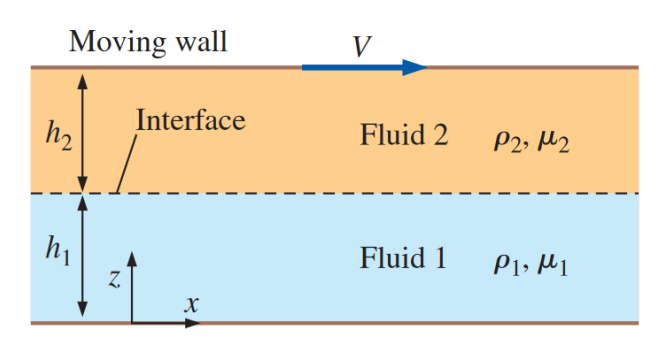
\includegraphics[width=0.5\textwidth]{Questions/Figures/Q3 Problem Diagram.png}
\end{figure}

\begin{enumerate}[label=\alph*)]
    \item \textit{List all the appropriate boundary conditions on both velocity and pressure. (Hint: There are six required boundary conditions)}
    \item \textit{Solve for the velocity field. (Hint: Split up the solution into two portions, one for each fluid. Generate expressions for $u_1$ as a function of $z$ and $u_2$ as a function of $z$)}
    \item \textit{Solve for the pressure field. (Hint: Again split up the solution. Solve for $P_1$ and $P_2$)}
    \item \textit{Let fluid 1 be water and let fluid 2 be unused engine oil, both at $80^\circ C$. Also, let $h_1 = 5.0 \, \text{mm}$, $h_2 = 8.0 \, \text{mm}$, and $V = 10.0 \, \text{m/s}$. Plot $u$ as a function of $z$ across the entire channel. Discuss the results.}
\end{enumerate}
\subsection*{Solution}
\subsection{}
The boundary conditions are 
\begin{table}[h]
    \centering
    \begin{tabular}{cc}
        \toprule
        Boundary Condition & Equation \\
        \hline
        No-slip at bottom plate & $u_1(0) = 0$ \\
        Continuity of velocity & $u_1(h_1) = u_2(h_1)$ \\
        No-slip at top plate & $u_2(h_1 + h_2) = V$ \\
        Continuity of pressure & $P_1(h_1) = P_2(h_1)$ \\
        Pressure at bottom & $P_1(0) = P_0$ \\
        Interface shear stress & $\tau_{12} = \mu_1 \frac{du_1}{dz} = \mu_2 \frac{du_2}{dz}$ \\
        \bottomrule
    \end{tabular}
\end{table}
\FloatBarrier
\subsection{}
We begin with the assumptions and their consequences:
\begin{table}[h]
    \centering
    \begin{tabular}{ccc}
        \toprule
        Number & Assumption & Consequence \\
        \hline
        \#1 & Steady flow & $\partial_t = 0$ \\
        \#2 & Incompressible flow & $\rho = \text{constant}$ \\
        \#3 & 2D flow & $u_y = 0$, $\partial_y \vec{v} = 0$ \\
        \#4 & Parallel flow & $w = 0$ \\
        \#5 & Gravity in $z$ & $g_z = -g$ \\
        \#6 & Fully Developed Flow & $\partial_x = 0$ \\
        \bottomrule
    \end{tabular}
\end{table}
\FloatBarrier
Starting with the continuity equation, we have
\begin{align*}
    \frac{\partial u_1}{\partial x} + \cancelto{\text{\#3}}{\frac{\partial v_1}{\partial y}} + \cancelto{\text{\#4}}{\frac{\partial w_1}{\partial z}} &= 0
\end{align*}
which implies that $u_1 = u_1(z)$. Now the momentum equation in the $x$ direction is
\begin{align*}
    \rho \left(\cancelto{\text{\#1}}{\frac{\partial u_1}{\partial t}} + u_1\cancelto{\text{Cont.}}{\frac{\partial u_1}{\partial x}} + \cancelto{\text{\#3}}{v_1 \frac{\partial u_1}{\partial y}} + \cancelto{\text{\#4}}{w_1 \frac{\partial u_1}{\partial z}}\right) &= -\cancelto{\text{\#6}}{\frac{\partial P_1}{\partial x}} + \mu_1 \left(\cancelto{\text{Cont.}}{\frac{\partial^2 u_1}{\partial x^2}} + \cancelto{\text{\#3}}{\frac{\partial^2 u_1}{\partial y^2}} + \frac{\partial^2 u_1}{\partial z^2}\right) - \cancelto{\text{\#5}}{\rho g_x}
\end{align*}
which simplifies to
\begin{align*}
    \frac{d^2 u_1}{dz^2} &= 0 \\
    \implies \frac{du_1}{dz} &= A \\
    \implies u_1 &= A z + B
\end{align*}
Since the assumptions hold for both fluid 1 and 2, the Navier-Stokes equation for fluid 2 is the same as for fluid 1. Thus, the velocity field for fluid 2 is
\begin{align*}
    \frac{du_2}{dz} &= C \\
    u_2 &= C z + D
\end{align*}
Applying the bottom plate boundary condition gives
\begin{align*}
    u_1(0) &= 0 = B \\
    \implies u_1 &= A z
\end{align*}
Applying the top plate boundary condition gives
\begin{align*}
    u_2(h_1 + h_2) &= V = C(h_1 + h_2) + D \\
    \implies D &= V - C(h_1 + h_2) \\
    \implies u_2 &= C z + V - C(h_1 + h_2)
\end{align*}
Applying the continuity of velocity gives
\begin{align*}
    u_1(h_1) &= u_2(h_1) \\
    A h_1 &= C h_1 + V - C(h_1 + h_2) \\ 
    &= C h_1 + V - C h_1 - C h_2 \\
    &= V - C h_2 \\
    \implies C &= \frac{V - A h_1}{h_2}
\end{align*}
Lastly, the shear stress condition gives 
\begin{align*}
    \mu_1 \frac{du_1}{dz} &= \mu_2 \frac{du_2}{dz} \\
    \mu_1 A &= \mu_2 C \\
    \implies A &= \frac{\mu_2}{\mu_1} C \\
    &= \frac{\mu_2}{\mu_1} \frac{V - A h_1}{h_2} \\
    \implies A &= \frac{\mu_2 V}{\mu_1 h_2 + \mu_2 h_1}
\end{align*}
Thus, the velocity field is
\begin{align*}
    u_1 &= \frac{\mu_2 V}{\mu_1 h_2 + \mu_2 h_1} z \\
    u_2 &= \frac{V - \frac{\mu_2 V}{\mu_1 h_2 + \mu_2 h_1} h_1}{h_2} z + V - \frac{V - \frac{\mu_2 V}{\mu_1 h_2 + \mu_2 h_1} h_1}{h_2}(h_1 + h_2)
\end{align*}
simplifying
\begin{verbatim}
syms mu1 mu2 V h1 h2 z
u2 = (V - (mu2*V*h1)/(mu1*h2 + mu2*h1))/h2*z ...
        + V - (V - (mu2*V*h1)/(mu1*h2 + mu2*h1))/h2*(h1 + h2);
u2 = simplify(u2)

>> u2 =
        (V*(h1*mu2 - h1*mu1 + mu1*z))/(h1*mu2 + h2*mu1)
\end{verbatim}
\begin{empheq}[box=\fbox]{align*}
    u_1 &= \frac{\mu_2 V z}{\mu_1 h_2 + \mu_2 h_1} \\
    u_2 &= \frac{V\mu_1z}{\mu_1 h_2 + \mu_2 h_1} + \frac{Vh_1\mu_2 - Vh_1\mu_1}{\mu_1 h_2 + \mu_2 h_1}
\end{empheq}

\subsection{}
Now the momentum equation in the $z$ direction is
\begin{align*}
    \rho_1 \left(\cancelto{\text{\#1}}{\frac{\partial w_1}{\partial t}} + u_1\cancelto{\text{Cont.}}{\frac{\partial w_1}{\partial x}} + \cancelto{\text{\#4}}{v_1 \frac{\partial w_1}{\partial y}} + \cancelto{\text{\#4}}{w_1 \frac{\partial u_1}{\partial z}}\right) &= -\frac{\partial P_1}{\partial z} + \mu_1 \left(\cancelto{\text{\#4}}{\frac{\partial^2 w_1}{\partial x^2}} + \cancelto{\text{\#4}}{\frac{\partial^2 w_1}{\partial y^2}} + \cancelto{\text{\#4}}{\frac{\partial^2 w_1}{\partial z^2}}\right) - \rho g_z
\end{align*}
which simplifies to
\begin{align*}
    \frac{dP_1}{dz} &= - \rho_1 g \\
    \implies P_1 &= -\rho_1 g z + E
\end{align*}
Since the assumptions hold for both fluid 1 and 2, the pressure field for fluid 2 is the same as for fluid 1. Thus, the pressure field for fluid 2 is
\begin{align*}
    P_2 &= -\rho_2 g z + F
\end{align*}
Using the boundary condition $P_1(0) = P_0$ gives
\begin{align*}
    P_{1}(0) &= P_0 = E \\
    \implies P_1 &= -\rho g z + P_0
\end{align*}
Lastly, the continuity of pressure gives
\begin{align*}
    P_1(h_1) &= P_2(h_1) \\
    -\rho_1 g h_1 + P_0 &= -\rho_2 g h_1 + F \\
    \implies F &= (\rho_2 - \rho_1) g h_1 + P_0
\end{align*}
Thus, the pressure field is
\begin{empheq}[box=\fbox]{align*}
    P_1 &= -\rho_1 g z + P_0 \\
    P_2 &= -\rho_2 g z + (\rho_2 - \rho_1) g h_1 + P_0
\end{empheq}
\FloatBarrier
\subsection{}
From the textbook,

\FloatBarrier
\begin{figure}[h]
    \centering
    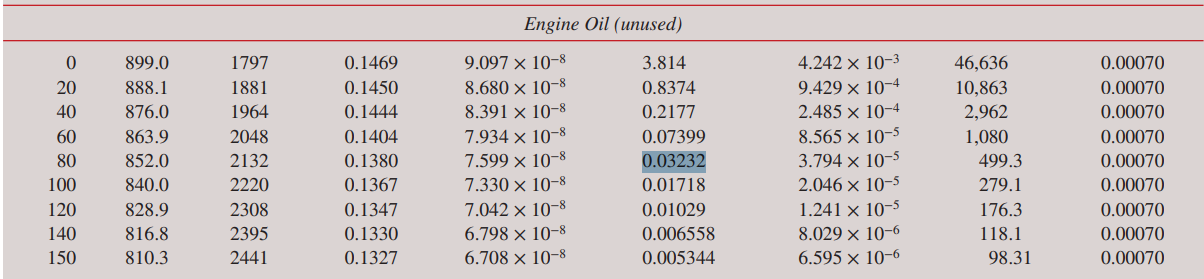
\includegraphics[width=0.8\textwidth]{Questions/Figures/Q3 Engine Oil Properties.png}
    \caption{Properties of Engine Oil at $80^\circ C$}
\end{figure}
\begin{figure}[h]
    \centering
    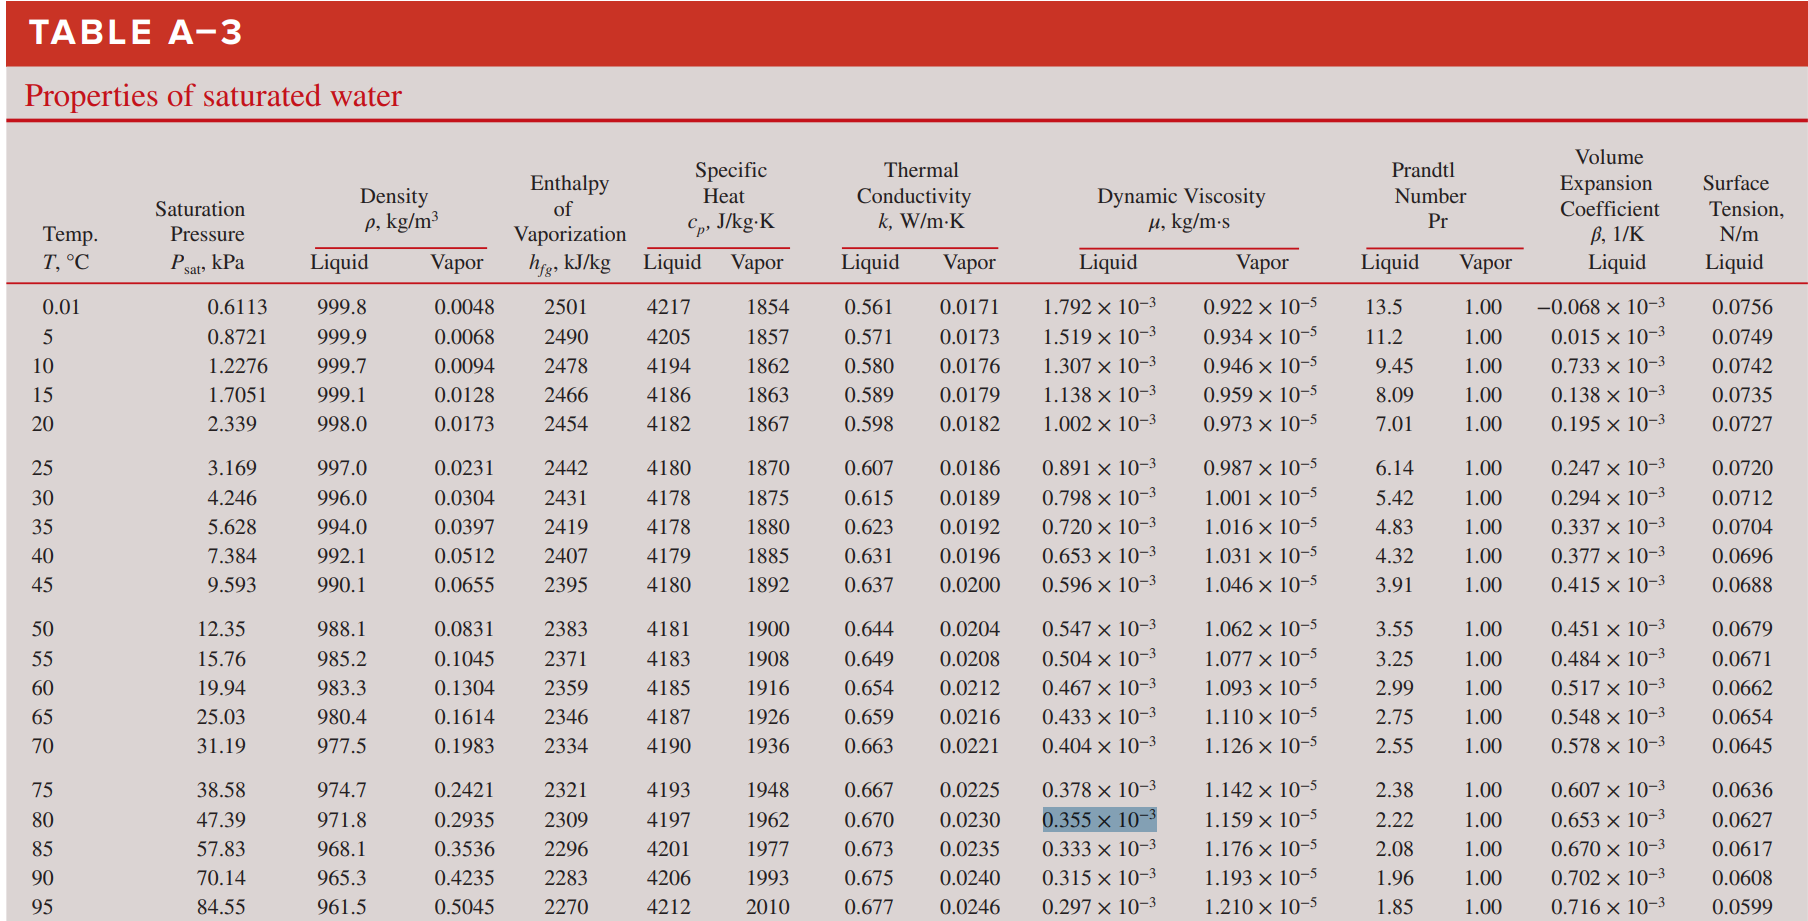
\includegraphics[width=0.8\textwidth]{Questions/Figures/Q3 Water Properties.png}
    \caption{Properties of Water at $80^\circ C$}
\end{figure}
From Desmos,
\begin{figure}[h]
    \centering
    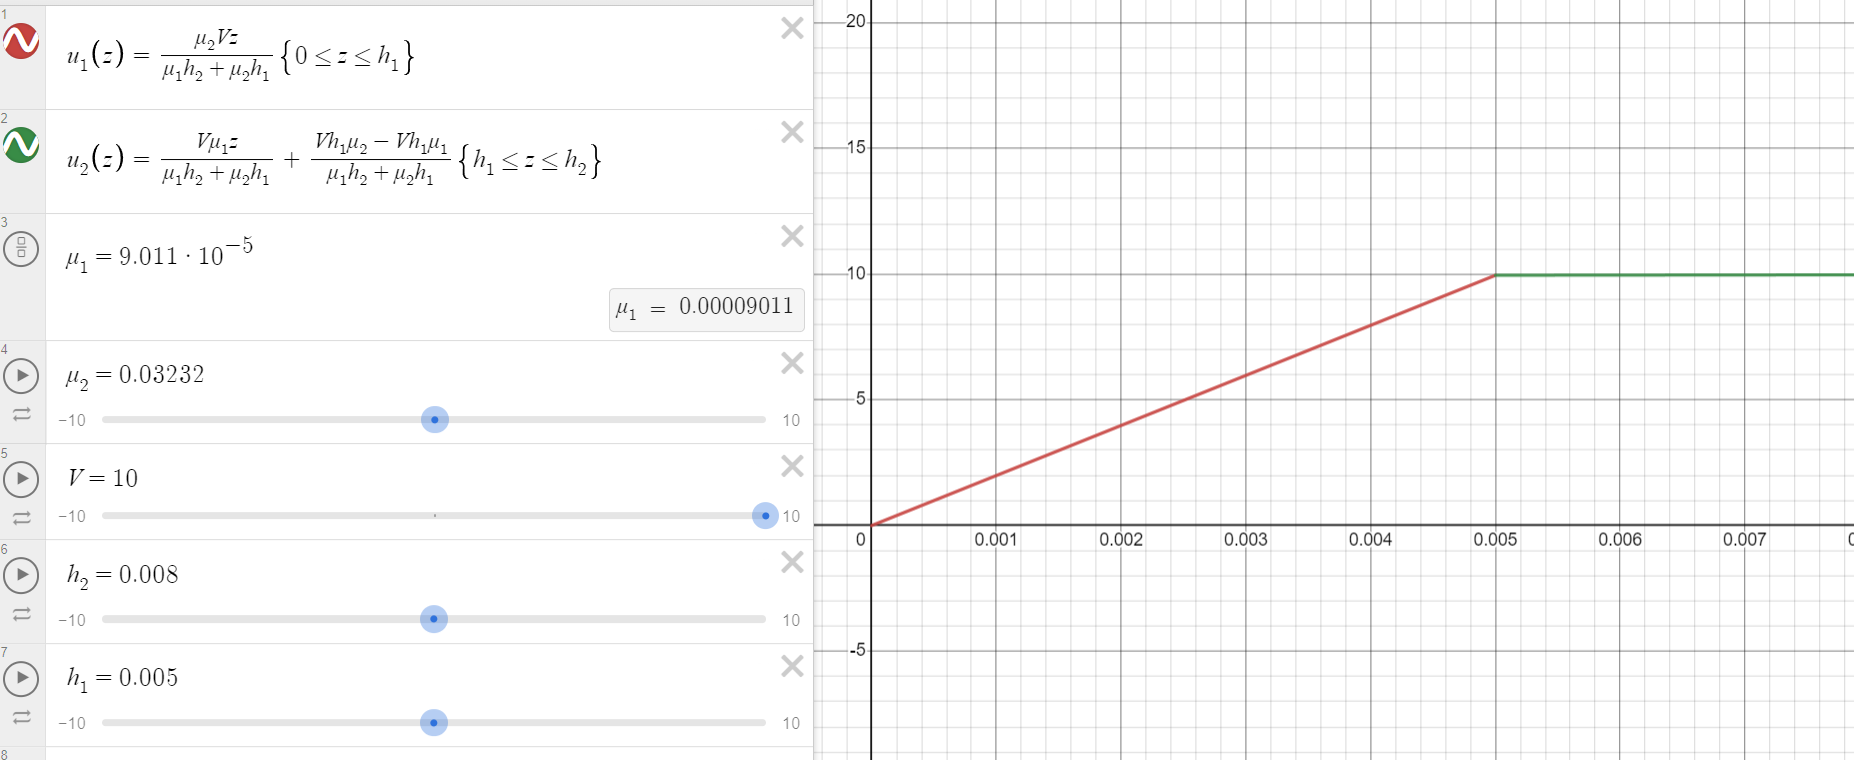
\includegraphics[width=1\textwidth]{Questions/Figures/Q3 Plot.png}
    \caption{$u$ as a function of $z$ across the entire channel}
\end{figure}
The flow is like two Couette flows connected to each other. The slope of the water is larger than the slope of the engine oil, which is expected since the viscosity of water is much lower than the viscosity of engine oil. The water's velocity nearly approaches the speed of the plate as it reaches the interface. 